\documentclass[12pt]{article}
\usepackage[margin=1.5cm]{geometry}
\usepackage{parskip}
\usepackage{amsmath}
\usepackage{amssymb}
\usepackage{amsfonts}
\usepackage{enumitem}
\usepackage{graphicx}
\usepackage{stmaryrd}
\graphicspath{ {./images/} }


\begin{document}
\begin{enumerate}[label=(\alph*)]
  \item
    A basic block is a sequence of instructions that will always execute sequentially, i.e. a sequence of instructions that has no branches except at the final instruction, and whose only entry point is the first instruction.

    Basic blocks are a useful IR for optimising compilers, since by converting a program into a graph of basic blocks, we have an IR that to some extent represents the control flow of a program. Having the control flow of a program readily available is useful for optimising compilers because it lets us easily reason about how a program might execute, what its possible paths are, or what instructions are guaranteed to execute at a particular point, for example.

  \item
    We first convert into 3-address code:

\begin{verbatim}
ADD r, x, 1
CMP y, 0
BNE else
MUL r, r, r
BR post
else:
SUB y, y, 1
MUL r, r, y
post:
ADD r, r, 1
RET r
\end{verbatim}

We then get the following flowgraph:

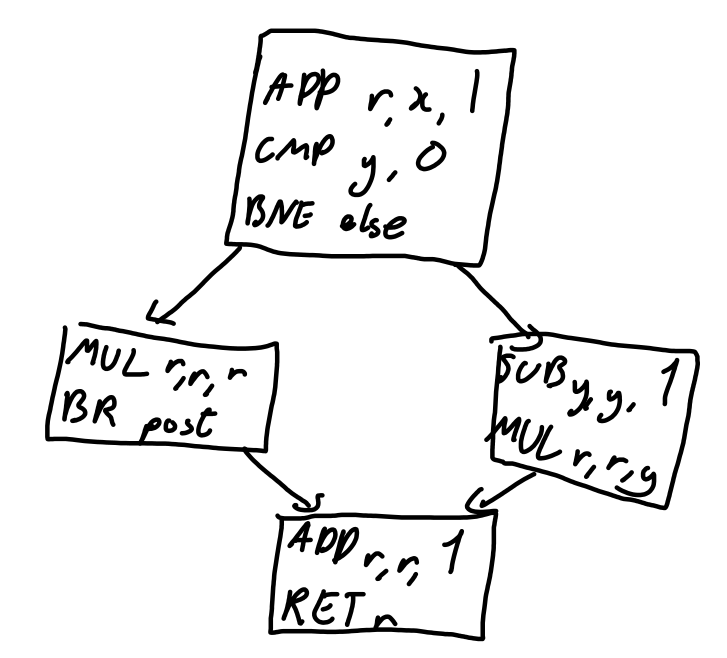
\includegraphics[scale=0.3]{flowgraph}

\item
  A program is in SSA form if every variable has at most one (static) assignment to it.

  To turn this flowgraph into SSA form, we would first need to ensure that the destination of each instruction is a different variable, by keeping a counter $i$ for each existing variable, and incrementing the counter upon assignment, changing the destination to $x_i$ instead of $x$, for example.

  We then need to insert pseudo instructions as a $\phi$ function at the basic block which has two predecessors, that chooses the correct version of each variable from the predecessors based on which branch we came from.

\item
  \begin{enumerate}[label=(\roman*)]

    \item
      A definition $m$ reaches $n$ if there exists some path through the flowgraph from $m$ to $n$ such that the variable to which $m$ assigns a value still has that value at entry to $n$.

    \item
      We design two complementary dataflow equations, analogously with available expression analysis.

      \[
        in-RD(n) = \bigcup_{p \in pred(n)} out-RD(p)
      .\] 

      \[
        out-RD(n) = in-RD(n) \setminus kill(n) \cup gen(n)$
      .\] 

      Where $kill(n)$ is the set of definitions that $n$ kills, i.e. those that it assigns to, and $gen(n)$ is the set of definitions that $n$ generates, i.e. those assignments that it makes.

      We combine these two into a single definition:

      \[
        RD(n) = \bigcup_{p \in pred(n)} \left(RD(p) \setminus kill(p) \cup gen(p)\right)
      .\] 

    \item
      We sketch the following algorithm:

\begin{verbatim}
RD[0..n] = {}
while (RD[] changes)
  for i = 0 to n do
    RD[i] = big_union(p in pred(n), RD[p] \ kill(p) U gen(p))
\end{verbatim}

The initialisation we do here is to initialise every set to the empty set. This ensures that we get the least solution possible.


      
  \end{enumerate}
        
    \end{enumerate}
\end{document}
